\documentclass[aspectratio=169, 10pt]{beamer}
\usefonttheme{serif}
\usepackage{graphicx}
\graphicspath{{./}{../figures/}{../../}}
\usepackage{booktabs}
\usepackage{xeCJK}
\usepackage{xcolor}
\setCJKmainfont{SimSun}

\usepackage{fontspec}
\newfontfamily\aeonik{Aeonik}

\title{MT-LNN: 受微管启发的液态神经网络}
\subtitle{打破内存墙的下一代长文本架构 \\ \textit{商业计划书 / Investor Pitch Deck}}
\author{\Huge \aeonik{Awareness}}
\date{2026年7月 \\[1em]
\footnotesize
\textbf{官网:} \url{https://awareliquid.ai} \\
\textbf{Paper:} \url{https://huggingface.co/EverestAn/MT-LNN} \\
\textbf{GitHub:} \url{https://github.com/everest-an/M1}
}


\usepackage{tikz}

\setbeamertemplate{navigation symbols}{}
\setbeamertemplate{footline}{
  \leavevmode%
  \hbox{%
  \begin{beamercolorbox}[wd=.333333\paperwidth,ht=2.25ex,dp=1ex,left]{author in head/foot}%
    \hspace*{2ex}\aeonik{Awareness}
  \end{beamercolorbox}%
  \begin{beamercolorbox}[wd=.333333\paperwidth,ht=2.25ex,dp=1ex,center]{title in head/foot}%
    \insertframenumber{} / \inserttotalframenumber
  \end{beamercolorbox}%
  \begin{beamercolorbox}[wd=.333333\paperwidth,ht=2.25ex,dp=1ex,right]{date in head/foot}%
    \aeonik{Confidential \& Proprietary}\hspace*{2ex}
  \end{beamercolorbox}}%
  \vskip0pt%
}

\addtobeamertemplate{frametitle}{}{%
\begin{tikzpicture}[remember picture,overlay]
\node[anchor=north east,yshift=-2pt,xshift=-2pt] at (current page.north east) {
\includegraphics[height=1.2cm]{logo.png}};
\end{tikzpicture}}

\begin{document}


\frame{\titlepage}

\begin{frame}{执行摘要}
\begin{itemize}
    \item \textbf{痛点：} 大语言模型（LLM）正撞上三堵物理之墙——\textbf{幻觉}（缺乏对物理世界的真实建模）、\textbf{成本爆炸}（KV 缓存的推理开销）、\textbf{模型体积}（被物理显存卡死的部署）。
    \item \textbf{方案：} MT-LNN 用连续时间液态神经网络（受大脑微管启发）取代 Transformer 的静态机制。
    \item \textbf{优势：} 恒定 $O(1)$ 内存占用，彻底消除 KV 缓存依赖；在消费级硬件上实现超长上下文（$>128K$ tokens）高性能推理。
    \item \textbf{本轮诉求：} 融资将架构从 1.5B 适配器阶段推进到原生 \textbf{2B 推理引擎}，并跑出支撑 7B 企业级运行的缩放曲线。
\end{itemize}
\end{frame}

\begin{frame}{我们解决的三大痛点}
\begin{itemize}
    \item \textbf{1. 幻觉（Hallucination）：} 大模型输出看似合理但物理上不可能的内容——它们没有对现实的内在建模。MT-LNN 的预测编码 + 空间世界模型预演在\textbf{源头}标红不合理结果。
    \item \textbf{2. 成本爆炸（Cost Explosion）：} 100 用户并发 10 万字文档需 $\sim$60 块 A100（约 \$100K/月）。MT-LNN 的 $O(1)$ 状态只需 \textbf{1 块 RTX 4090}（约 \$200/月）——\textbf{成本降低约 500 倍}。
    \item \textbf{3. 模型体积 / 显存墙（Model Size）：} Transformer 的 KV 缓存内存 $O(N)$、计算 $O(N^2)$ 膨胀。MT-LNN 携带\textbf{恒定 0.381 MB 状态}——1M 上下文下比 KV 缓存小 \textbf{8{,}063 倍}，可部署于手机、穿戴设备与边缘 MCU。
\end{itemize}
\end{frame}

\begin{frame}{成本爆发的元凶：KV 缓存}
\begin{itemize}
    \item \textbf{强迫式的记录引擎：} Transformer 架构如同强制录像机，预测下一个词时，必须把过去所有词的特征放入显存中（即 KV Cache）。
    \item \textbf{复杂度灾难：} 随着文本增长，内存复杂度为 $O(N)$，计算复杂度飙升至 $O(N^2)$。
    \item \textbf{实例：} 仅仅 10 万字的上下文，就会瞬间塞满一台昂贵的 A100 GPU；更不用提在只有十几 GB 内存的手机或端侧设备部署，这在物理上是不可能的。
\end{itemize}
\end{frame}

\begin{frame}{成本爆炸 vs. 完美扩展机制}
\begin{itemize}
    \item Transformer 架构依赖不断膨胀的 KV 缓存，在处理超长上下文时导致服务成本飙升以及巨大的内存压力。
    \item MT-LNN 采用紧凑的循环隐状态与微管神经启发的选择性动态机制，完美控制了运算时的内存增长。
    \item \textbf{商业化意义：} 大幅降低了私有化/本地化部署和端侧及边缘设备（Edge Devices）场景的落地阻力与门槛。
\end{itemize}
\begin{center}
    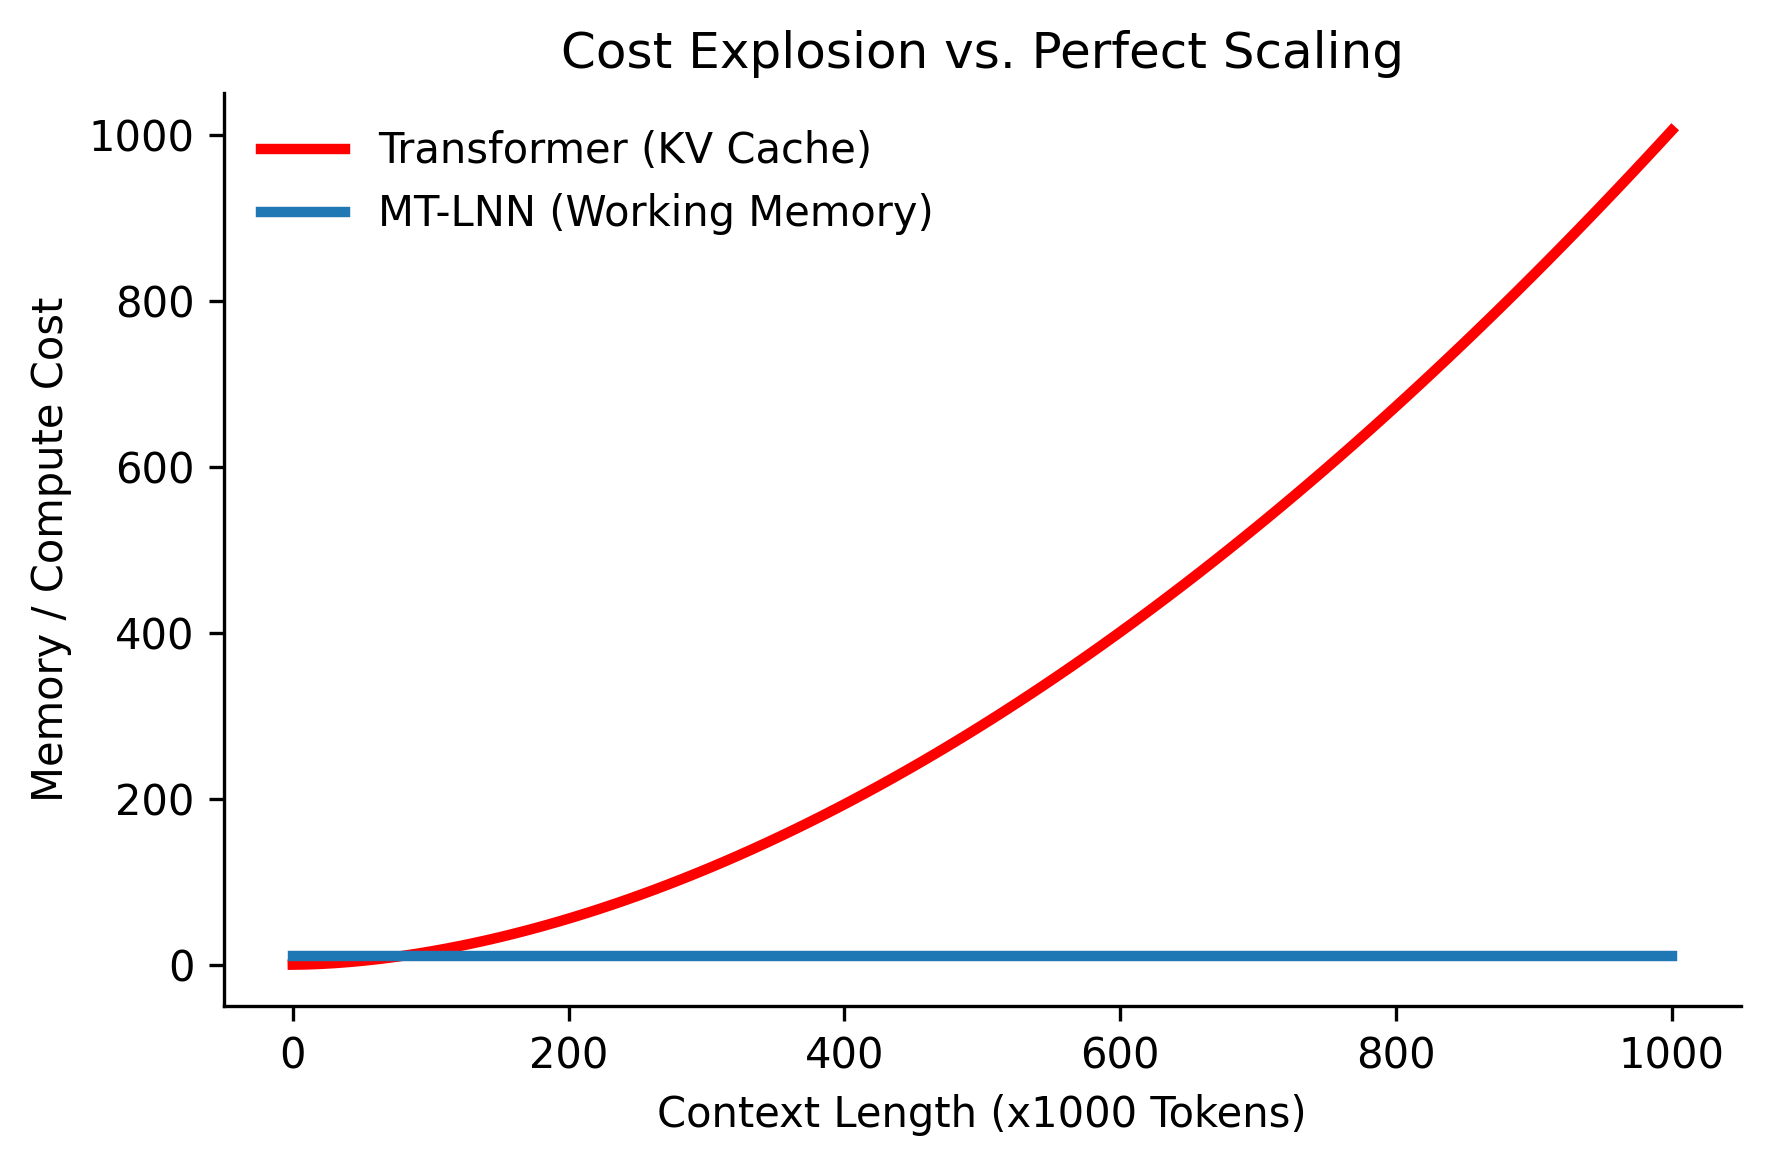
\includegraphics[height=0.45\textheight]{cost_explosion.png}
\end{center}
\end{frame}

\begin{frame}{我们的方案：MT-LNN 架构登场}
\begin{columns}
\begin{column}{0.6\textwidth}
\textbf{预测编码与 $O(1)$ 微管液态系统：}
\begin{itemize}
    \item \textbf{重构前馈与缓存墙：} 抛弃标准 Transformer 中耗费显存的静态 FFN 和 $O(T)$ KV 缓存，替换为 13 个平行的多尺度连续时间网络以及 \textbf{$O(1)$ 工作记忆衰减矩阵}。
    \item \textbf{内置解释性与跳过机制：} 引入动态计算跳过（Endogenous Compute Skipping）指数级节省显存算力。内置因果链与自我监控提取头，打破大模型黑盒困境。
    \item \textbf{一整套认知栈，而非单个混合器：} \textbf{GWT 全局工作区瓶颈}（专家通道竞争共享广播）、\textbf{睡眠周期巩固}（NREM 式合成把短期痕迹压缩为持久结构）、以及跨窗口/跨会话携带 key$\to$value 绑定的\textbf{快权重记忆}。
\end{itemize}
\end{column}
\begin{column}{0.4\textwidth}
\centering
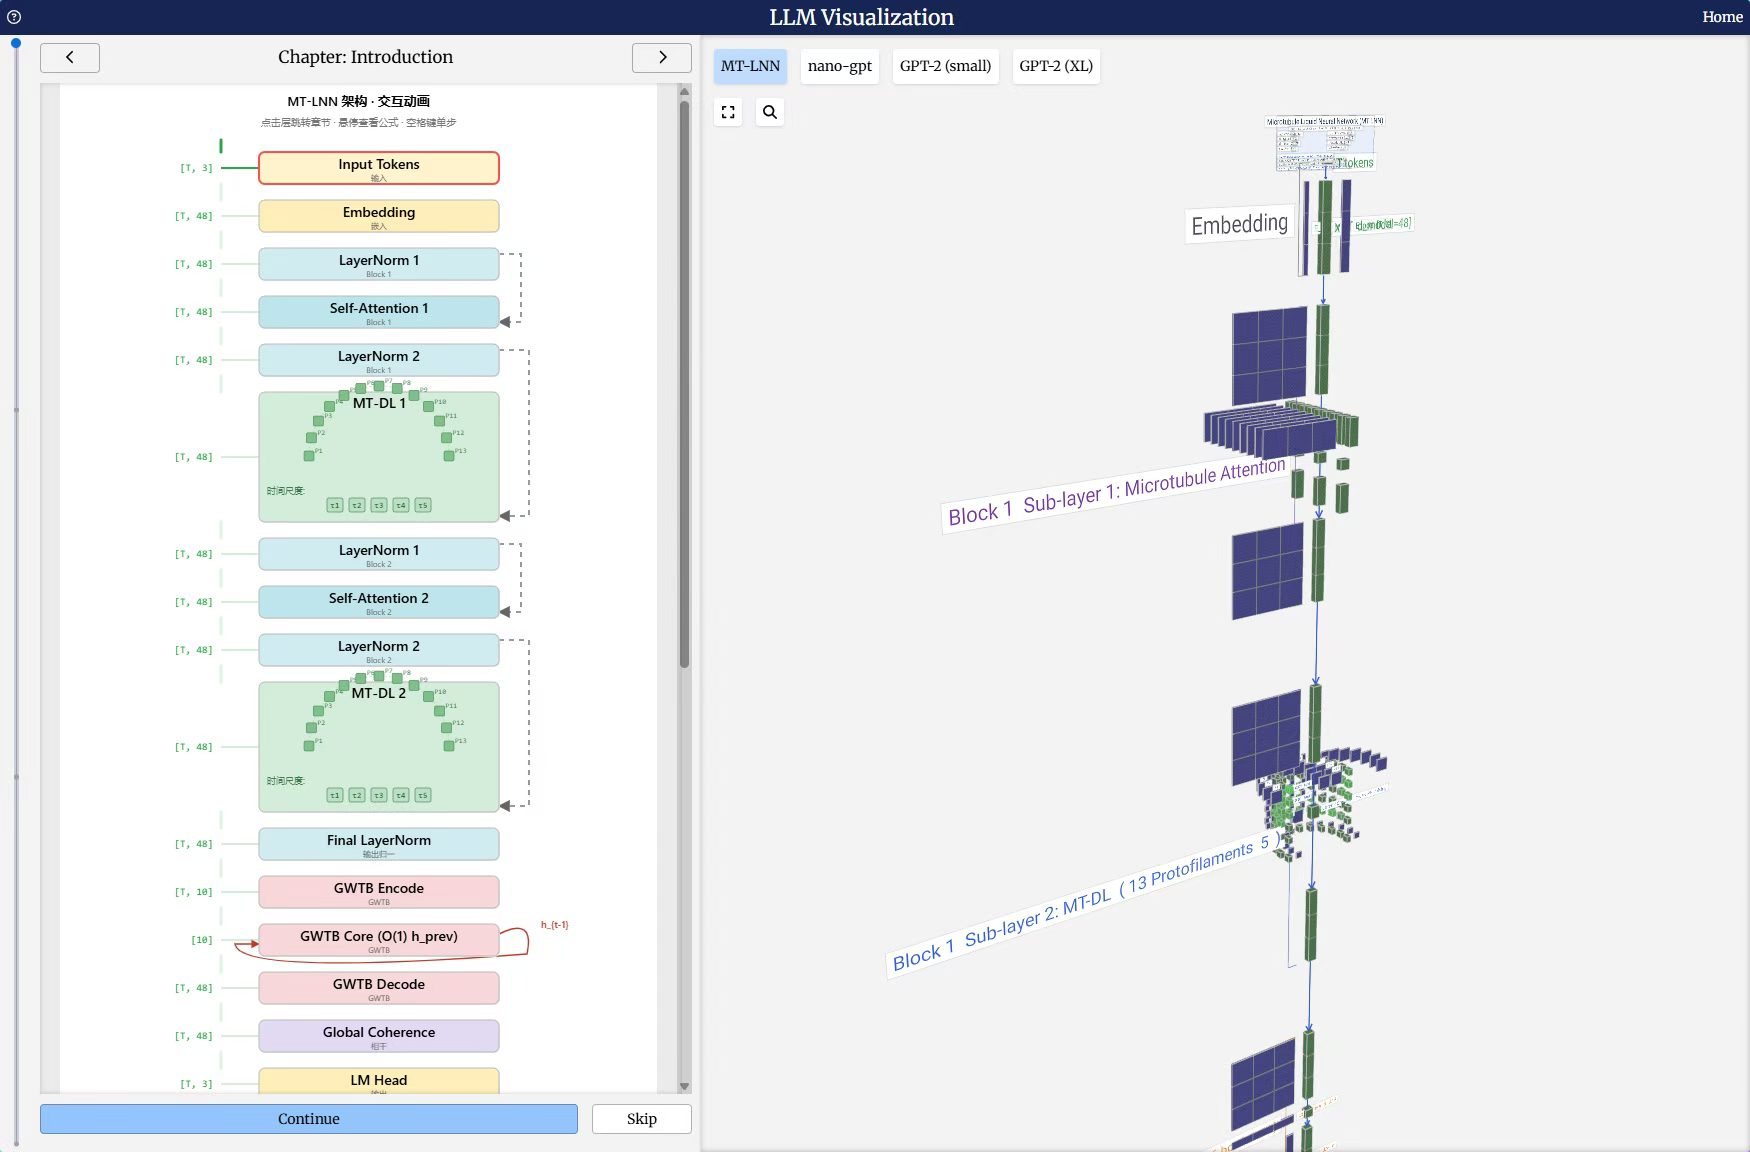
\includegraphics[width=0.9\textwidth,height=0.55\textheight,keepaspectratio]{stracture.jpg}
\end{column}
\end{columns}
\end{frame}

\begin{frame}{生物学启示：人脑机制}
\begin{itemize}
    \item \textbf{不记录每个像素：} 人类大脑绝对不会，也不可能记住十年来每个画面的精确像素和所有细节。
    \item \textbf{工作记忆与选择性遗忘：} 我们的认知高度依赖于“工作记忆”（滞存核心线索）与“选择性遗忘”（抛弃无关噪音）。
    \item \textbf{AI 的盲区：} 现有的标准 LLM 仅仅是庞大的纯数学矩阵乘法，缺乏此类动态时间流逝机制，也未体现全局工作区（GWT）等意识级别的信息整合路径。
\end{itemize}
\end{frame}

\begin{frame}{双产品线：M1 + O1}
\small
\begin{columns}[T]
\begin{column}{0.5\textwidth}
\textbf{M1（M 系列）—— 认知慢思维}
\begin{itemize}\itemsep=0.3em
    \item 混合架构：冻结的开源基座（如 TinyLlama-1.1B）+ 我们训练的 MT 液态适配器，参数开销仅 $\sim$1\%。
    \item 在保留基座全部质量的同时叠加 \textbf{GWT 工作区 + 睡眠巩固 + EWC 持续学习}。
    \item 独有优势：\textbf{跨窗口 / 跨会话联想召回} —— 0.56，而冻结注意力 / LoRA 结构性为 \textbf{0.000}。
    \item \textbf{服务场景：} 云端 / GPU / 私有化企业部署。
\end{itemize}
\end{column}
\begin{column}{0.5\textwidth}
\textbf{O1（O 系列）—— 边缘快思维}
\begin{itemize}\itemsep=0.3em
    \item 无注意力、从零训练（48M--125M），液态 ODE 动力学，毫秒级延迟。
    \item \textbf{真正的 O(1) 推理内存：} 携带状态从 512 到 1{,}048{,}576 tokens 恒定 \textbf{0.381 MB}，同级 KV 缓存则涨到 \textbf{3{,}072 MB}（相差 8{,}063 倍）。
    \item \textbf{服务场景：} 智能穿戴、车载、工业流式传感器 —— MCU 级硬件。
\end{itemize}
\end{column}
\end{columns}
\vspace{0.4em}
{\footnotesize 两条产品线共享同一套认知栈 —— GWT 工作区、预测编码、液态时间常数。在线演示：\url{https://awareliquid.ai}}
\end{frame}

\begin{frame}{M1 深度：上下文窗口被丢弃后仍然记得}
\begin{itemize}
    \item \textbf{一个注意力机制在结构上做不到的任务：} 先存入 key$\to$value 事实，\emph{把整个 KV 缓存 / 上下文窗口丢掉}，再提问。冻结注意力与 LoRA 得分 \textbf{0.000} —— 信息彻底消失。
    \item \textbf{MT-LNN 快权重记忆：跨窗口平均召回 0.56}（3 随机种子）。消融掉快权重矩阵后召回塌到 0.008 —— 状态\emph{就是}记忆本体。
    \item \textbf{跨会话持久化：} $(F, z)$ 状态落盘快照、在全新进程中恢复，\textbf{逐位无损} —— “跨会话记住你”是架构属性，不是外挂 RAG 数据库。
    \item \textbf{诚实边界：} 这是情景式 key$\to$value 记忆，而非长上下文语言建模增益（窗口外语言建模为实测零收益）—— 我们明确说清它是什么、不是什么。
\end{itemize}
\end{frame}

\begin{frame}{O1 深度：恒定内存流式推理}
\begin{itemize}
    \item \textbf{已验证至 100 万 Tokens（2026-07-19）：} 在无注意力的 O 系列上，推理携带状态在\textbf{上下文增长 2048 倍}（512 $\to$ 1{,}048{,}576）的条件下\textbf{恒定为 0.381 MB}，而同等 Transformer 的 KV 缓存线性增长至 \textbf{3{,}072 MB}——差距 \textbf{8{,}063 倍}，为实测而非外推。
    \item \textbf{算子压缩：} 1000 Tokens —— 传统 KV 需要 1020 KB；O1 状态流模式仅需恒定的 \textbf{4.1 KB}。
    \item \textbf{稀疏共振：} Top-$k$ 门控剔除沉寂通道 —— 纯 CPU 吞吐从 \textbf{6161 提升到 6645 tok/s}（top-$k{=}1$ 时 $+7.9\%$，输出偏差仅 0.3\%）。
    \item \textbf{非均匀采样鲁棒性（NASA 电池）：} 80\% 时间步缺失下，mt\_lnn 仅退化 \textbf{+7.7\%}，而 LSTM \textbf{+31.1\%} / GRU \textbf{+32.8\%} —— 液态 ODE 原生属性，非补丁。
\end{itemize}
\end{frame}

\begin{frame}{官方同尺寸对比 1：选择性拷贝（200K 参数）}
\begin{columns}
\begin{column}{0.55\textwidth}
\textbf{超长噪声插入测试 ($T=229$)：}
\begin{itemize}
    \item \textbf{长度压力测试：} 随着文本长度和无关噪声的增加，所有模型的逐序列完全匹配率都会下降。在公平的全序列解码下，$T=229$ 时 Transformer 基线降至 \textbf{10.9\%}，传统 LNN 为 \textbf{17.2\%}。
    \item \textbf{MT-LNN 优势随长度扩大：} 凭借动态选择性过滤与隐状态遗忘机制，MT-LNN 在该长度下仍以 \textbf{21.9\%} 领先，约为 Transformer 的 \textbf{2$\times$}。
\end{itemize}
\vspace{0.5em}
\textbf{在同等极小参数量 (200K) 评测下，MT-LNN 在各长度上的逐序列召回均领先：$T=32$ 时较 Transformer 适度领先约 1.3$\times$（89.5\% vs 67.6\%），并随序列增长扩大至约 2$\times$。}
\end{column}
\begin{column}{0.45\textwidth}
\centering
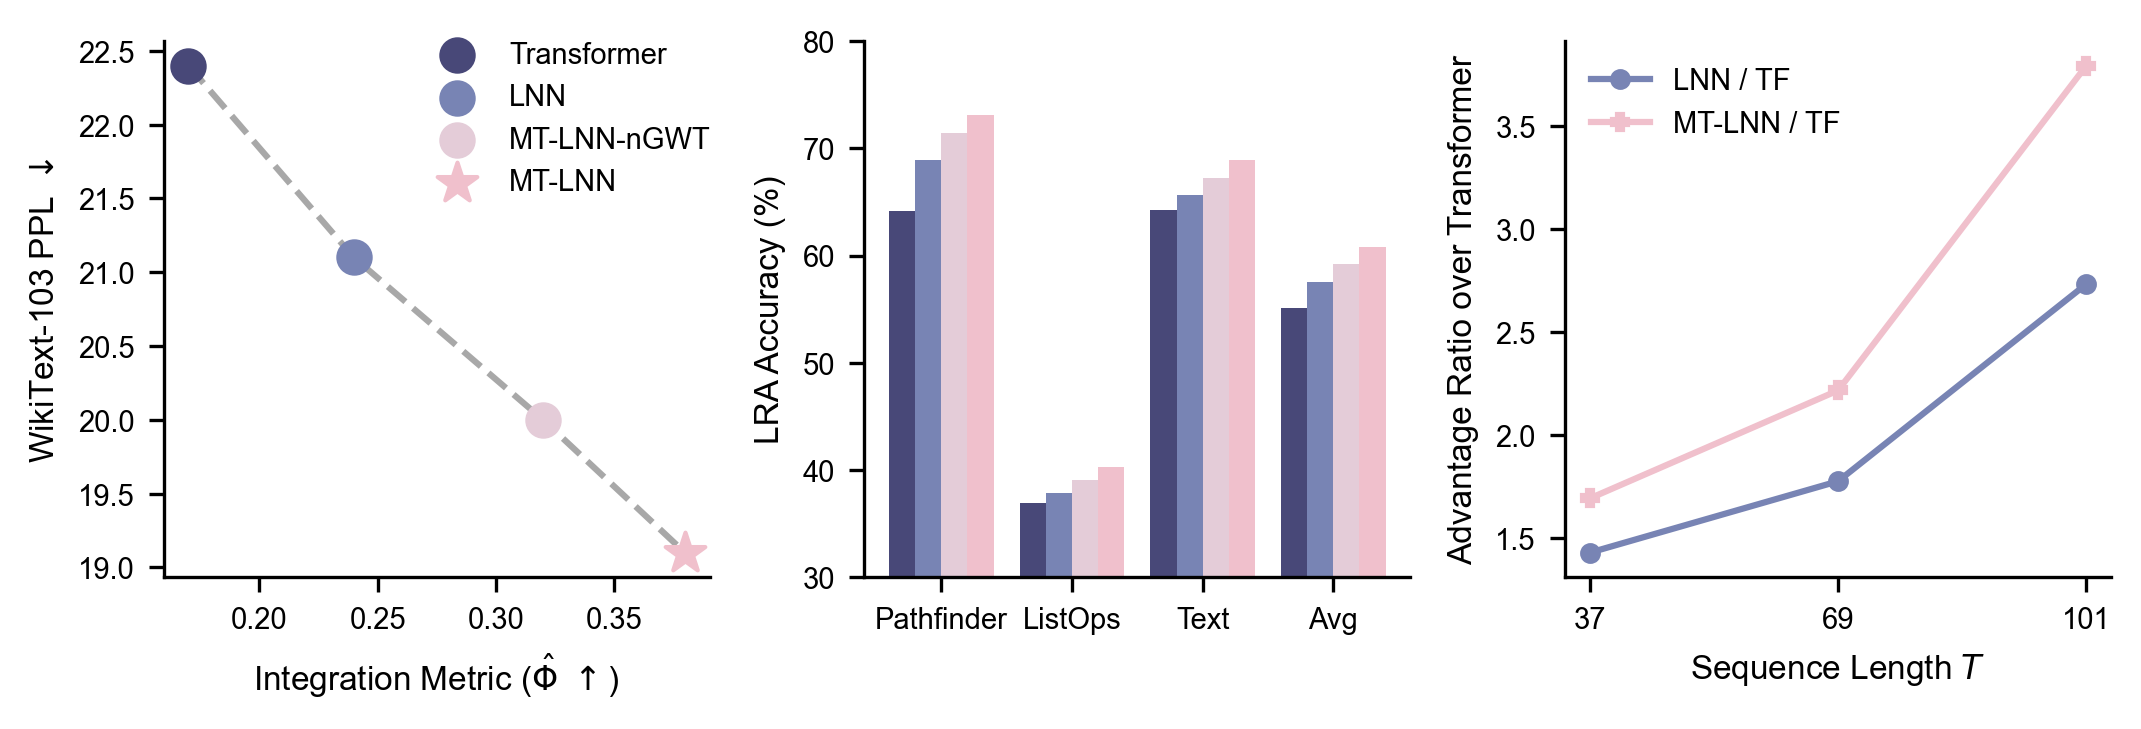
\includegraphics[width=0.95\textwidth]{fig_experiments.png}
\end{column}
\end{columns}
\end{frame}

\begin{frame}{官方同尺寸对比 2：125M 收敛 \& O(1) 内存}
\small
\begin{itemize}\itemsep=0.3em
    \item \textbf{125M 级、WikiText-103 从零训练至收敛（20K 步，3 随机种子，fp32）：}
    \begin{center}
    \begin{tabular}{lccc}
    \toprule
    \textbf{模型} & \textbf{参数量} & \textbf{验证 PPL} & \textbf{稳定性} \\
    \midrule
    MT-LNN & 126.0M & 88.93 $\pm$ 0.33 & 稳定（无 NaN） \\
    简单 Transformer & 142.1M & 94.14 $\pm$ 0.78 & 稳定 \\
    现代 Transformer & 144.1M & 78.86 $\pm$ 0.25 & 稳定 \\
    \bottomrule
    \end{tabular}
    \end{center}
    \item \textbf{诚实定位：} MT-LNN 比简单基线好 5.5\%；现代 Transformer 在原始 PPL 上领先 11.3\%。\textbf{原始语言建模质量不是我们的取胜点。}
    \item \textbf{同尺寸下我们赢在哪里：} O(1) 推理内存 —— 1M 上下文下 \textbf{0.381 MB vs 3{,}072 MB（8{,}063 倍）}，这是任何 Transformer 配置都无法消除的结构性差异。
\end{itemize}
\end{frame}

\begin{frame}{已验证的落地场景（已发布或已实测）}
\small
\textbf{来自架构本身：}
\begin{itemize}\itemsep=0.4em
    \item \textbf{电池管理（NASA PCoE 数据集）：} 流式电芯健康度回归，携带状态仅 \textbf{2.6 KB}；在 \textbf{80\% 样本缺失下仅退化 +7.7\%}，而 LSTM +31.1\%、GRU +32.8\% —— 对非均匀采样的鲁棒性是液态 ODE 的原生属性，不是补丁。
    \item \textbf{智能穿戴 —— 开源唤醒词（O1-Sound）：} 常开关键词识别，\textbf{5.12 KB 恒定状态}；无云端依赖，MCU 级硬件毫秒响应。
    \item \textbf{工业哨兵（DualSpeedSentry）：} 快反应 + 慢思考、数学上限安全输出、容器化开箱即用。
\end{itemize}
\vspace{0.2em}
\textbf{来自文档问答适配器}（独立产品线 —— 围绕\emph{冻结}基座模型的检索/压缩层）：
\begin{itemize}\itemsep=0.4em
    \item \textbf{金融文档：} 多域标注评测集 \textbf{91.7\%（44/48）}，每题仅约 \textbf{1.3 次模型调用、约 2.8k tokens}，全程本地私有化。179 项测试全绿。
\end{itemize}
\vspace{0.2em}
{\footnotesize 在线演示与复现脚本：\url{https://awareliquid.ai} · GitHub \texttt{everest-an/M1}}
\end{frame}

\begin{frame}{应用场景 1：合规企业（法律 / 金融 / 政企）}
\begin{itemize}
    \item \textbf{B 端目标客户痛点吻合：}
        顶尖律所面临海量千页卷宗的溯源；风投/审计财团对无尽财报报表的数据对齐；或大型科技厂商进行的底层百万行老旧祖传代码库盘查检越。
    \item \textbf{三要素完美匹配：} MT-LNN 精准满足这部分客户迫切需求的三个必要条件：1. 超长篇幅大批量吞吐能力。2. 绝对的私有合规和不联网隔离。3. 基于极低硬件投入的一次性低成本本地部署。
    \item \textbf{金融文档已实测：} 多域标注评测集 \textbf{91.7\%（44/48）}，全程本地私有化，每题约 1.3 次模型调用。
\end{itemize}
\end{frame}

\begin{frame}{应用场景 2：边缘与 IoT 设备}
\begin{itemize}
    \item \textbf{解决物理芯片发热与功耗瓶颈：} 模型不仅体积小，而且对内存读写的极速优化使得我们能将其无缝嵌入到功耗受限的可穿戴 AR 交互外设和车载中枢内。
    \item \textbf{全天候陪伴式流信息处理：} 现存主流 AI 无法承载几十小时全时段开启音视频输入捕捉，而 MT-LNN 随时间递进的连续动态吸收机制天然适用这类连绵不断的外界数据流场景。
    \item \textbf{实测足迹：} O1 携带状态 \textbf{5.12 KB}（唤醒词）/ \textbf{2.6 KB}（电池健康度）—— 运行于 MCU 级硬件、毫秒级延迟、无需云端。
\end{itemize}
\end{frame}

\begin{frame}{应用场景 3：工业监测与安防}
\begin{itemize}
    \item \textbf{可部署的“哨兵”（DualSpeedSentry）：} 日常用便宜的“条件反射”盯着，只有真出现异常苗头时才\textbf{唤醒“深度思考”}——\textbf{大幅省算力}。
    \item \textbf{掉线也不失控：} 信号中断时，它会凭惯性“续推一会儿”或干脆\textbf{安全停机}，绝不乱动。
    \item \textbf{输出永远在安全范围内：} 动作幅度被\textbf{数学上限死}，保证不会输出超出机械极限的危险指令。
    \item \textbf{可直接部署：} 配套服务化接口（带验收测试）+ 容器打包与运维工具，\textbf{开箱即可上线}。
\end{itemize}
\end{frame}

\begin{frame}{竞争格局矩阵}
\begin{table}[]
\resizebox{\textwidth}{!}{
\begin{tabular}{lccccc}
\toprule
\textbf{特性} & \textbf{MT-LNN} & \textbf{GPT-4/Claude} & \textbf{Mamba/RWKV} & \textbf{Liquid AI (LFM)} & \textbf{本地 Llama} \\
\midrule
超长上下文 & \textcolor{green}{支持} & \textcolor{green}{支持} & \textcolor{orange}{退化} & \textcolor{green}{支持} & \textcolor{red}{失败 (OOM)} \\
隐私 / 本地部署 & \textcolor{green}{支持} & \textcolor{red}{不支持 (云端)} & \textcolor{green}{支持} & \textcolor{orange}{部分} & \textcolor{green}{支持} \\
低硬件要求 & \textcolor{green}{支持 (MacBook)} & \textcolor{red}{不支持 (A100)} & \textcolor{green}{支持} & \textcolor{green}{支持} & \textcolor{red}{不支持} \\
恒定内存 $O(1)$ & \textcolor{green}{支持} & \textcolor{red}{不支持} & \textcolor{green}{支持} & \textcolor{green}{支持} & \textcolor{red}{不支持} \\
跨会话原生记忆 & \textcolor{green}{支持} & \textcolor{red}{不支持} & \textcolor{red}{不支持} & \textcolor{red}{不支持} & \textcolor{red}{不支持} \\
端侧持续学习 & \textcolor{green}{支持\textsuperscript{*}} & \textcolor{red}{不支持} & \textcolor{red}{不支持} & \textcolor{red}{不支持} & \textcolor{orange}{仅 LoRA} \\
\bottomrule
\end{tabular}
}
\end{table}
\vspace{0.2em}
{\footnotesize \textsuperscript{*}EWC、经验回放与生成式做梦重放均已在小规模上多种子验证；尚未在 $\geq$1B 规模复现。\\
\textbf{对比 Liquid AI：} 他们做商用推理效率优化；AwareLiquid 聚焦\textbf{认知连续性与终身学习} —— 在线权重更新 + 跨会话持久状态，而非仅靠上下文内学习。}
\end{frame}

\begin{frame}{成本-能力定位（AA 斩杀线方法论）}
\begin{columns}
\begin{column}{0.52\textwidth}
\centering
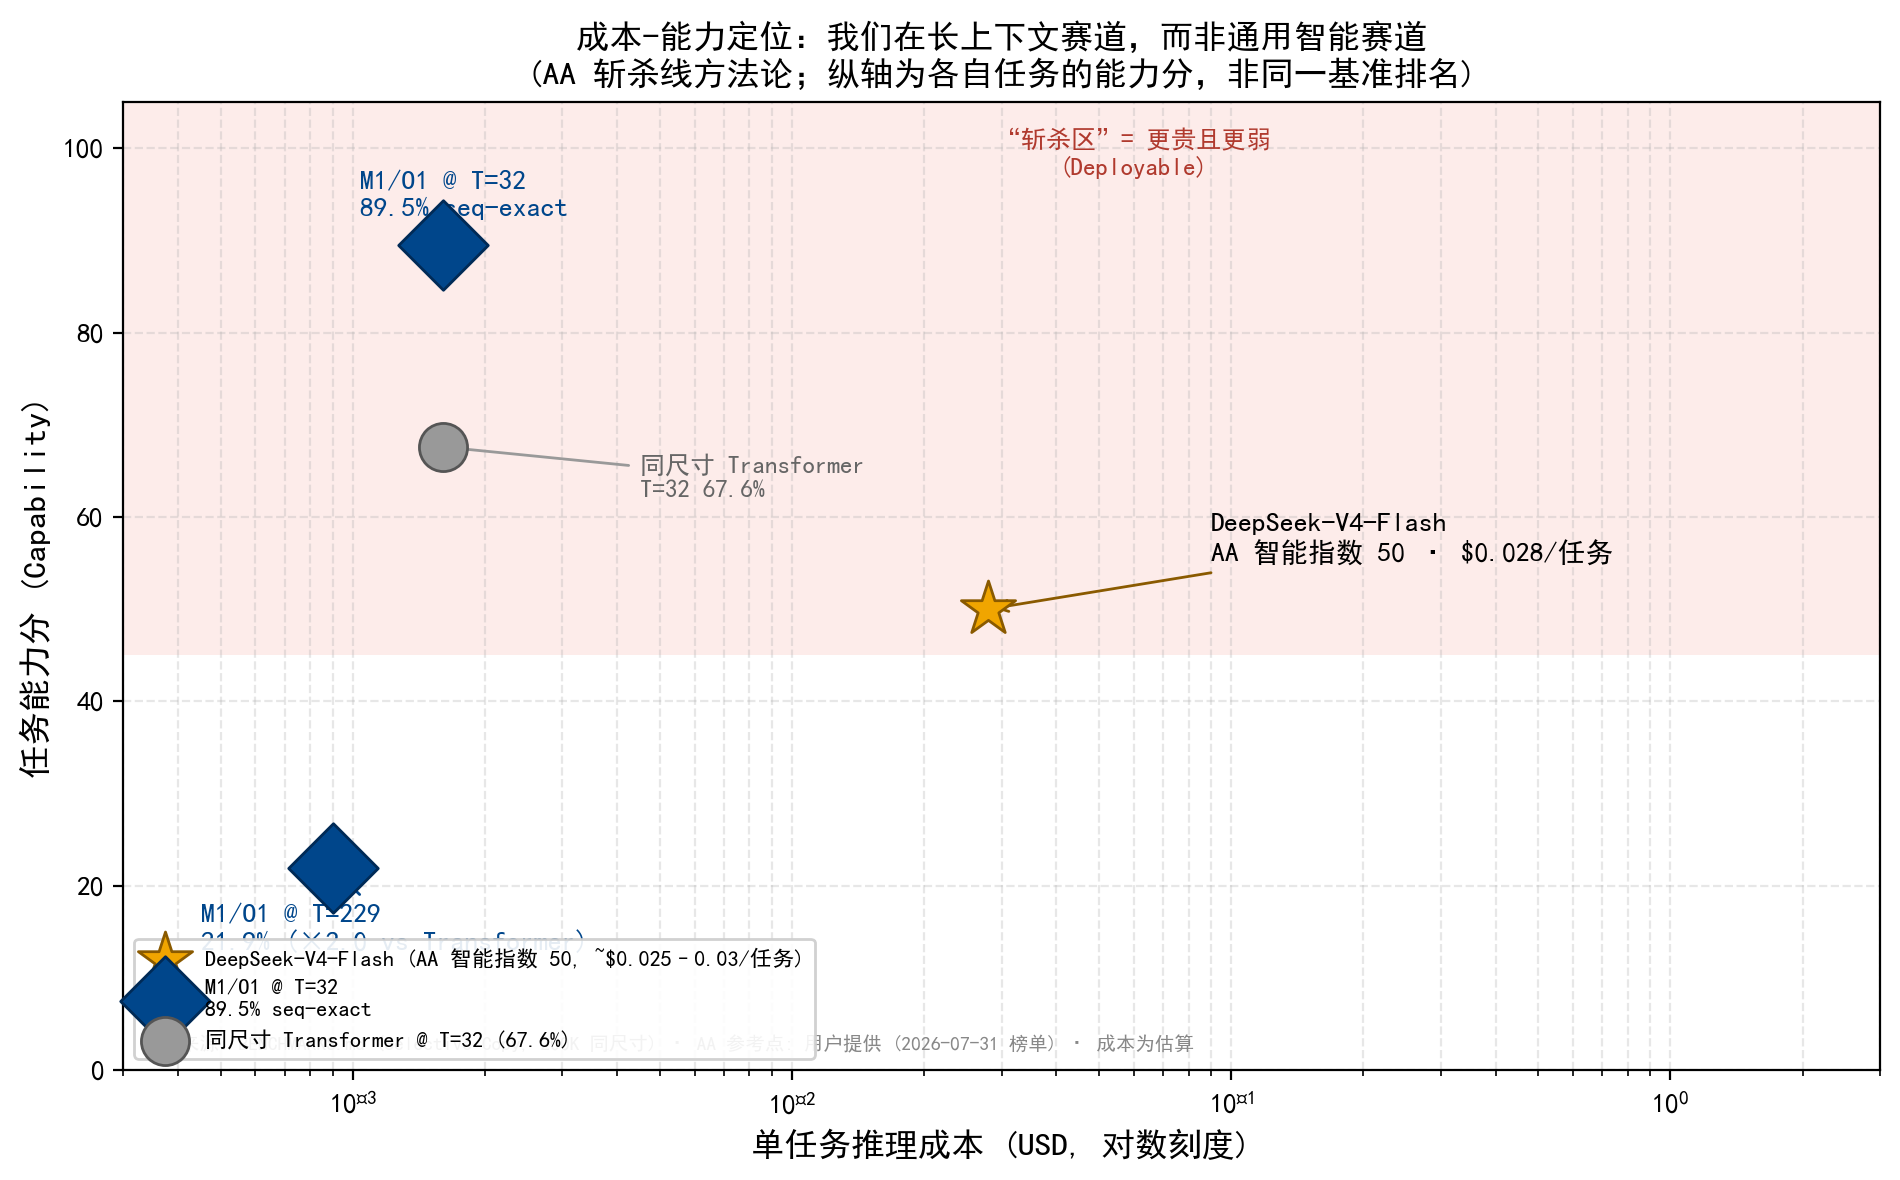
\includegraphics[width=\textwidth,height=0.52\textheight,keepaspectratio]{fig_cost_capability_positioning.png}
\end{column}
\begin{column}{0.48\textwidth}
\centering
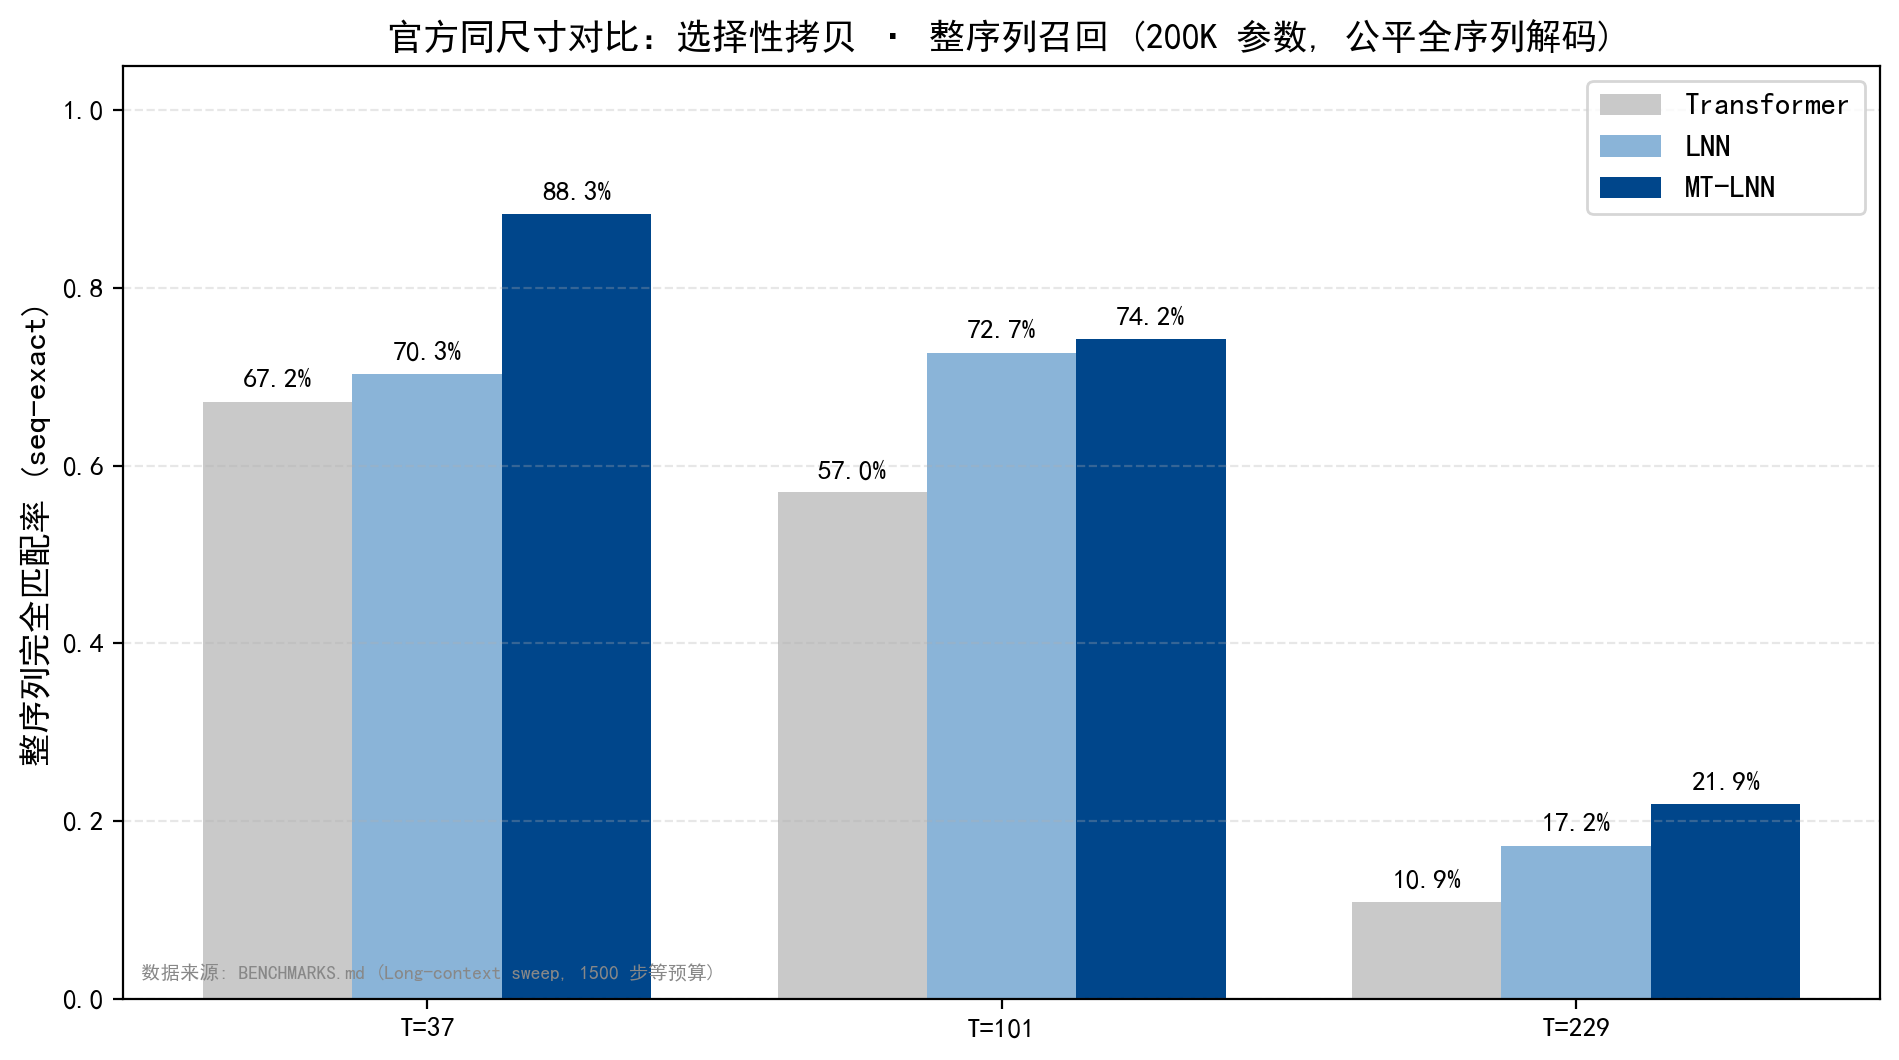
\includegraphics[width=\textwidth,height=0.52\textheight,keepaspectratio]{fig_selective_copy_samesize.png}
\end{column}
\end{columns}
\vspace{0.2em}
{\footnotesize
\textbf{诚实的定位：} 我们不在通用智能指数上竞争（MMLU / Agent 套件是为 AGI 级模型设计的；48M--1.1B 模型在那里接近随机）。我们在\textbf{长上下文 + 端侧成本}赛道竞争：同尺寸 200K 参数下，MT-LNN 在每个长度的整序列召回均领先（$T{=}32$ 89.5\% vs 67.6\%；$T{=}229$ 达 $\times$2.0），配合 $O(1)$ 内存（1M 上下文 0.381 MB vs 3{,}072 MB）——单任务成本比云端 API 低 2--3 个数量级。
}
\end{frame}

\begin{frame}{市场规模与定位}
\begin{itemize}
    \item \textbf{TAM（总可寻址市场）\$120B+：} 全球生成式 AI 与 LLM 推理市场，涵盖云服务、企业应用与边缘智能。
    \item \textbf{SAM（可服务市场）\$45B：} 企业数据处理、法律审查、财务审计、数据隐私至上的本地优先 AI 软件市场。
    \item \textbf{SOM（可获得市场）\$2.5B+：} 被云端 API 隐私风险完全阻断、急需低成本私有化超长上下文方案的 B2B 组织。
\end{itemize}
\begin{columns}
\begin{column}{0.5\textwidth}
\centering
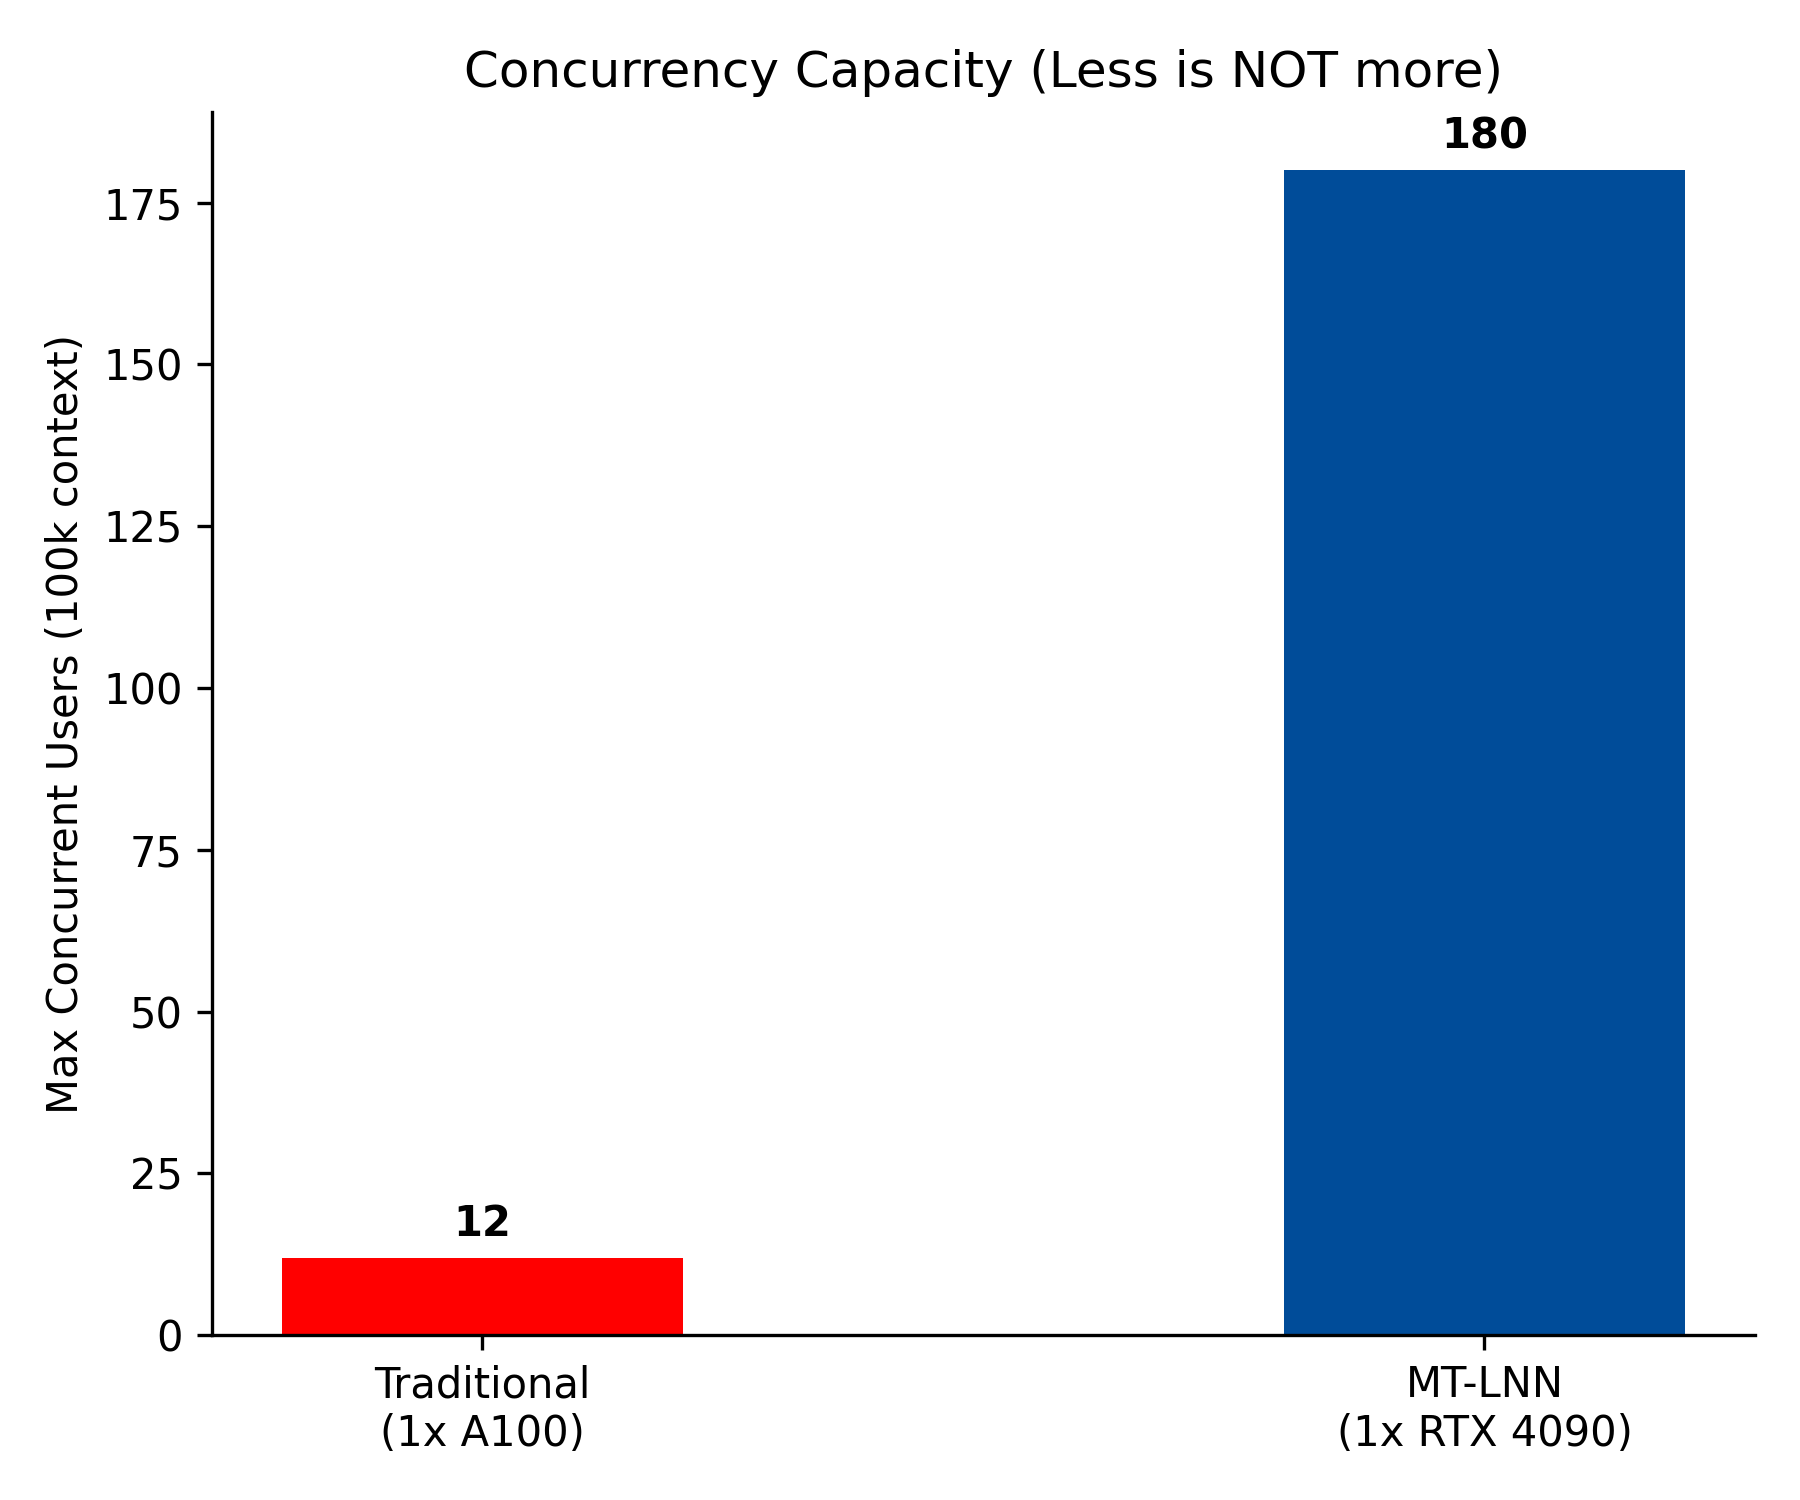
\includegraphics[width=0.95\textwidth,height=0.3\textheight,keepaspectratio]{concurrency.png}
\end{column}
\begin{column}{0.5\textwidth}
\centering
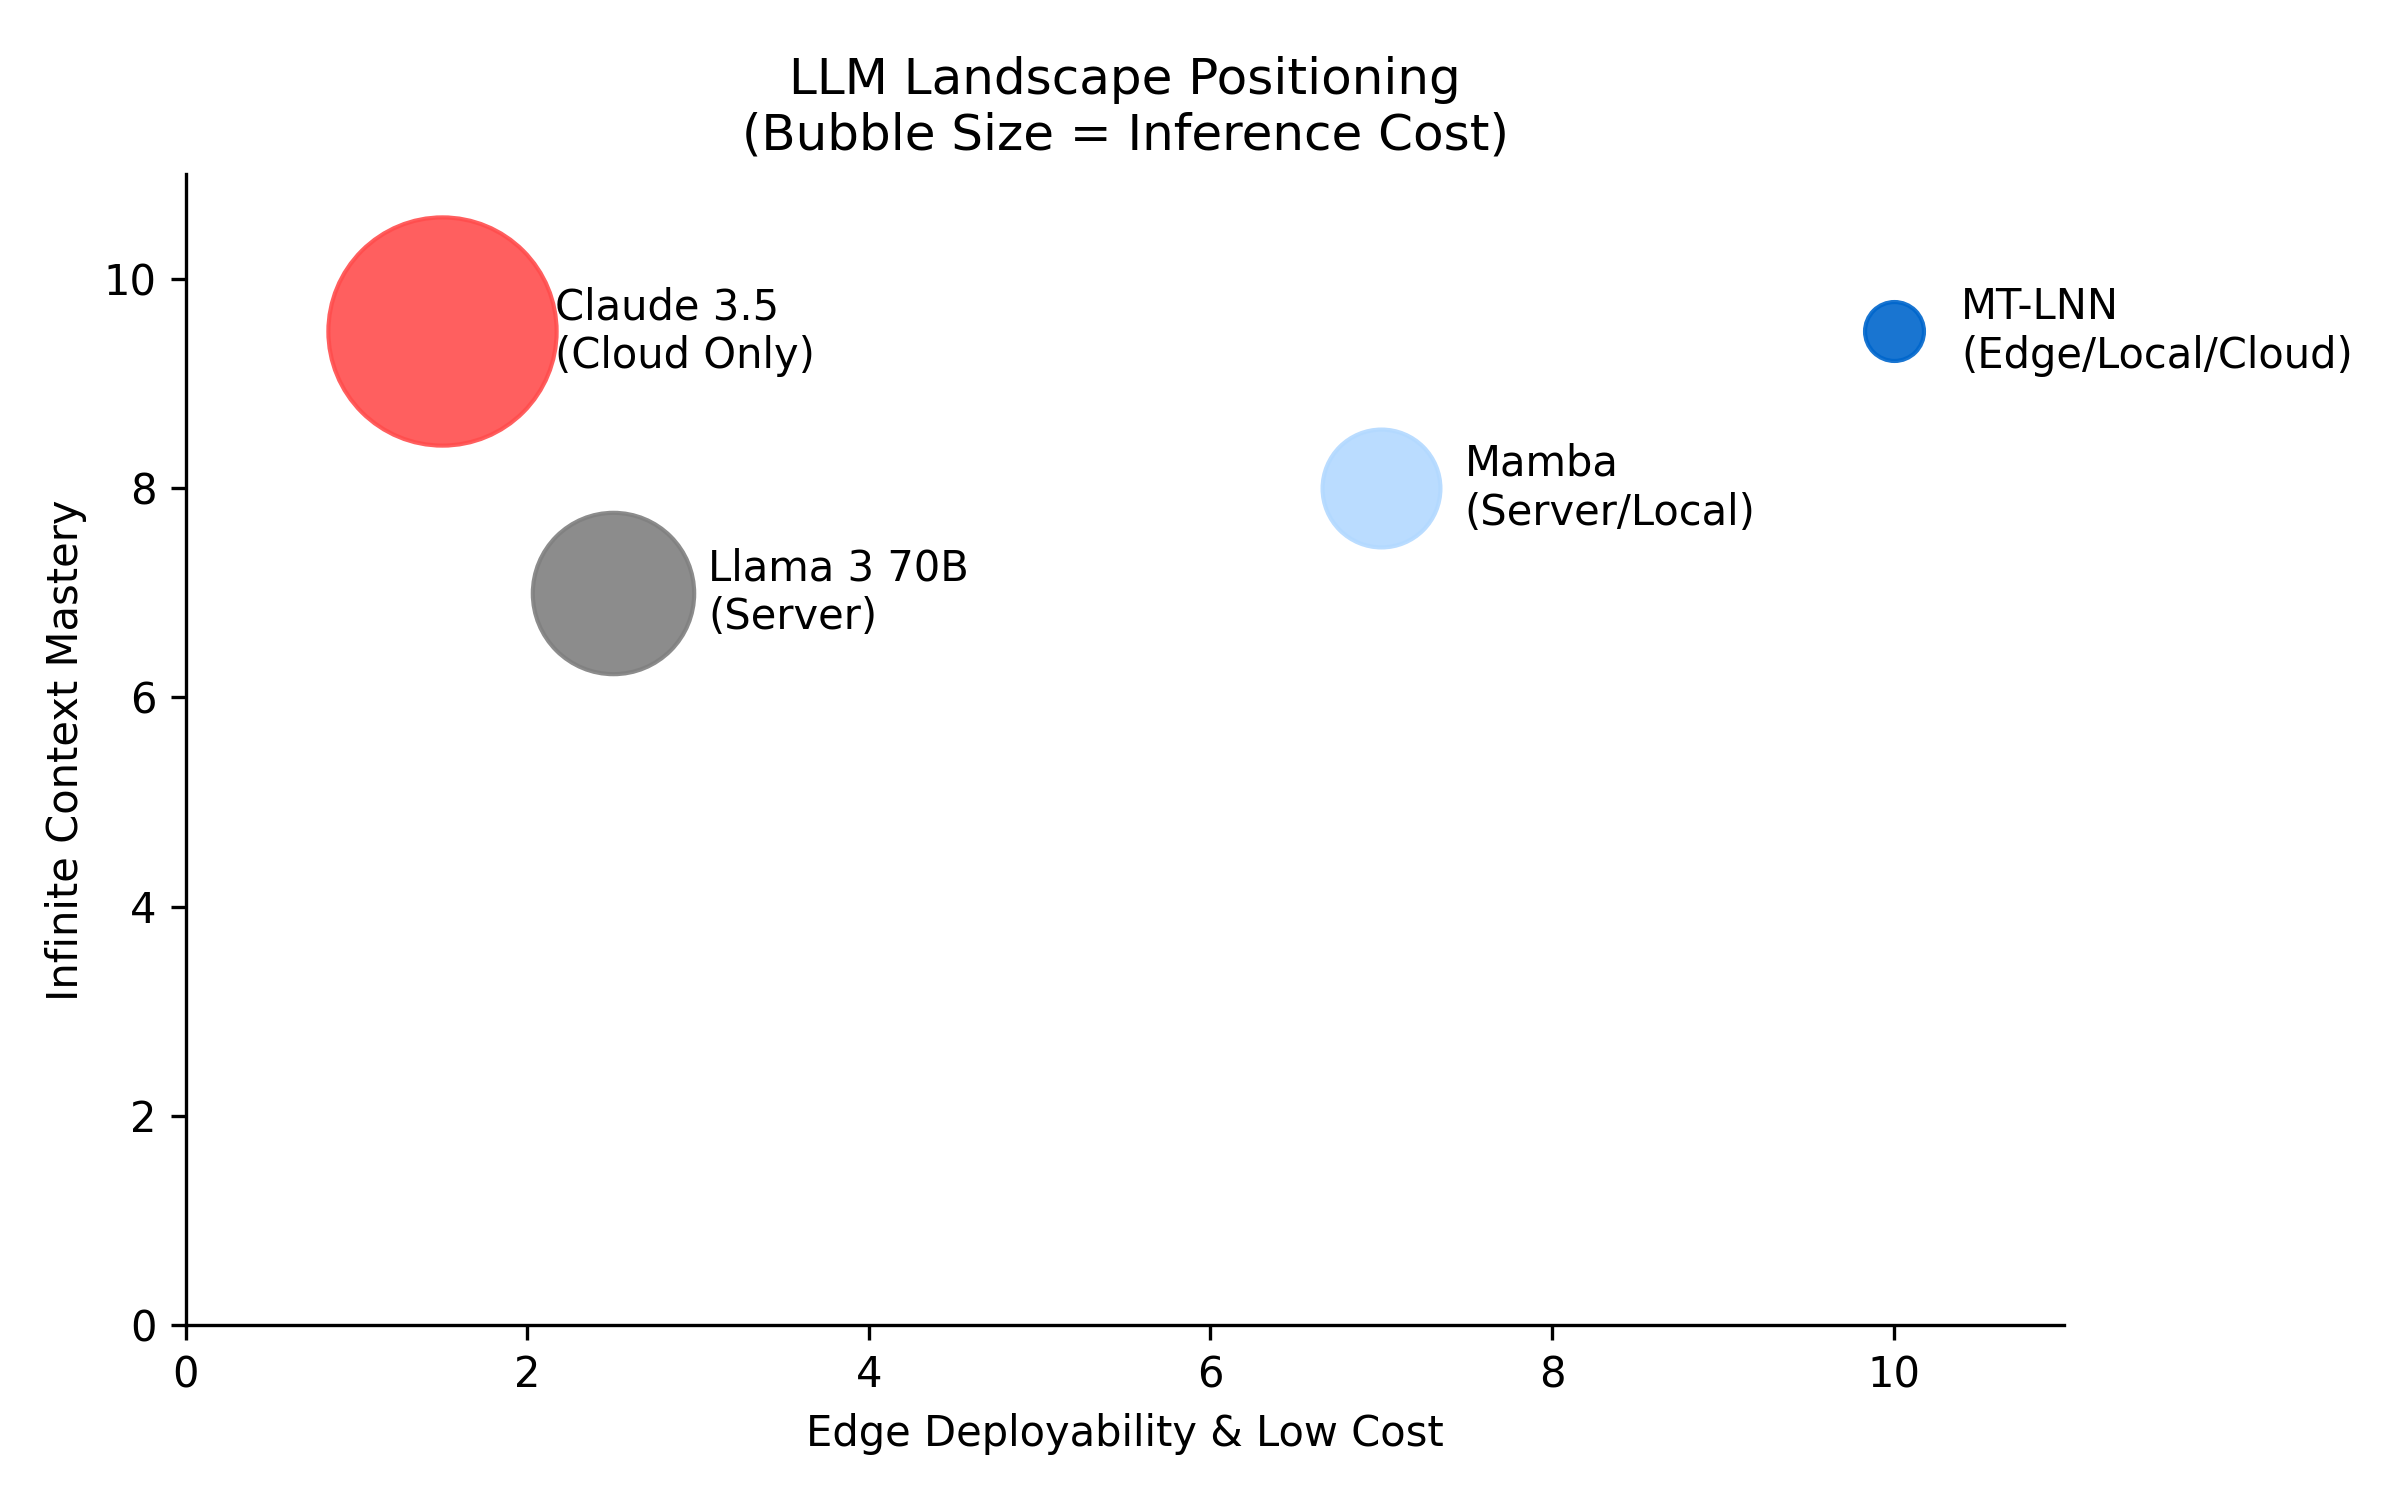
\includegraphics[width=0.95\textwidth,height=0.3\textheight,keepaspectratio]{landscape.png}
\end{column}
\end{columns}
\end{frame}

\begin{frame}{商业模式：双收入流}
\begin{itemize}
    \item \textbf{1. B2B 企业授权（本地部署）：}
    \begin{itemize}
        \item 向强监管行业（法律、金融、国防）直接销售私有授权。
        \item 直接部署到客户内部服务器。100\% 本地化，0\% 数据泄露风险。
    \end{itemize}
    \item \textbf{2. 高效云端 API：}
    \begin{itemize}
        \item 推理成本比 Transformer API 低 $\sim$90\%，可在保持巨大利润空间的同时大幅低于市场领导者定价。
    \end{itemize}
\end{itemize}
\end{frame}

\begin{frame}{市场进入（GTM）策略}
\begin{itemize}
    \item \textbf{阶段 1：开源社区锚点：} 发布 1.5B 组件到 OSS。赢得开发者心智、引爆技术评测、建立草根工程漏斗。
    \item \textbf{阶段 2：定向 B2B 试点部署：} 与 5 家顶级律所和基金启动私有概念验证（PoC）。仅凭文档解析节省的工时证明 ROI。
    \item \textbf{阶段 3：API 市场：} 推出自助开发者门户，提供高吞吐、廉价、长上下文推理封装，替代标准 OpenAI/Anthropic 管道。
\end{itemize}
\end{frame}

\begin{frame}{核心技术路线与 18 个月展望}
\begin{enumerate}
    \item \textbf{一阶段验证期 (当前)：} 在极小参数级模型（如挂载架构至 1.5B 参数量级规模）下，初步获得行业内长文本测评榜单领先与学术验证，并吸引第一梯队种子与社区开发者讨论。
    \vspace{0.5em}
    \item \textbf{二阶段原生推理引擎 (随后的 6-12 个月内)：} 蒸馏优先，先在 350M--1B 上用 $\mu$P 验证缩放曲线，再训练完全原生的 \textbf{2B 混合架构}（液态核心 + 稀疏注意力）与学习型记忆控制器 —— 知识外置于检索，本体只做推理。同期与初期 B 端合作伙伴共建落地闭环。\textbf{7B 由实测缩放曲线决定是否启动，不预设。}
    \vspace{0.5em}
    \item \textbf{三阶段迈向下一代泛化多模态基座 (未来 18 个月以上)：} 跨越多模态，使用超千亿宏大数据集参与大规模通用联合训练。并用该极致常数时间效能最终推动更高度的泛化 AGI 理解引擎构建计划底座。
\end{enumerate}
\end{frame}

\begin{frame}{核心团队：AwareLiquid}
\small
\begin{itemize}\itemsep=0.4em
    \item \textbf{Everest An —— 创始人 / 核心架构师}（AI 记忆系统专家）。前 \textbf{IPFS Athna} 核心成员，主导企业级分布式数据库底层架构；曾任 \textbf{Outliers Fund} 投资管理经理（主投 \textbf{Dfinity}、\textbf{Harmony}、\textbf{Analog}、\textbf{Quantstamp}）；多次斩获全球以太坊黑客马拉松冠军。
    \item \textbf{Eric —— CTO。} \textbf{NEMO protocol} 与 \textbf{STABLE} 架构师，统筹 M 系列 / O 系列模型与服务栈全线工程。
    \item \textbf{博士研究团队 —— 香港理工大学 (PolyU)：} \textbf{Wang Yuxiang、Huang Xinhui、Kenser、Gloria} —— 方向覆盖连续时间动力学、记忆巩固与评测体系。
    \vspace{0.3em}
    \item \textbf{顾问：}
    \begin{itemize}
        \item \textbf{Pan Kai 教授} —— 香港理工大学教授。
        \item \textbf{Yi Zhou} —— Stable Diffusion 架构师。
    \end{itemize}
\end{itemize}
\end{frame}

\begin{frame}{融资方案与阶段目标 (The Ask)}
\begin{columns}
\begin{column}{0.5\textwidth}
\textbf{本轮诉求：Seed / A 轮 - \$3.5M}
\vspace{0.5em}
\begin{itemize}
    \item 启动原生 \textbf{2B 推理引擎}训练（蒸馏优先，$\mu$P 验证）。
    \item 组建成熟的 GTM 和企业级销售团队。
    \item \textbf{12个月里程碑（非营收承诺）：}
    \begin{itemize}\footnotesize
        \item 与 $\geq$ 10 家企业/研究机构签署合作备忘录 / PoC。
        \item 其中 3--5 家转为付费 design partner，建立可验证的付费需求信号。
        \item 发布第一个生产环境可用 2B 检查点 + 实测三规模缩放曲线 + 公开 benchmark 报告。
    \end{itemize}
\end{itemize}
\end{column}
\begin{column}{0.5\textwidth}
\textbf{资金使用占比：}
\begin{itemize}
    \item \textbf{50\% 算力与预训练：} 租赁 H100 / A100 集群跑 2B 基座训练，以及决定是否放大的缩放曲线各档位。
    \item \textbf{30\% LNN 核心研究：} 拓充连续时间动力学 (LTC ODE)、Orch-OR 启发选择机制、工作记忆 GWTB 方向的研究人员，差异化的技术周边护城河在这里。
    \item \textbf{20\% GTM 与市场：} B 端客户销售 + 社区 / 论文 / 品牌。
\end{itemize}
\end{column}
\end{columns}
\end{frame}

\begin{frame}{我们真正的技术护城河}
\small
\begin{itemize}\itemsep=0.4em
    \item \textbf{架构原创性（最深的一层）：} MT-LNN 本身——连续时间 LTC ODE + Orch-OR 启发的选择机制 + GWTB 工作记忆三件套——是我们的原创架构，论文在投稿中。架构本身是不可被快速复现的原创资产。
    \item \textbf{可复现的训练 recipe 与跨基座经验：} 从 Qwen-0.5B 到 Qwen-3B、Llama 多个基座上的 adapter 训练数据、超参与消融报告均已沉淀在仓库。后来者即使拿到架构，也需数月 reproduce 这一套经验。
    \item \textbf{Benchmark 与评测体系 + OSS 飞轮：} 大海捞针 / 选择性拷贝 / O(1) 内存压力测试 / 稀疏共振消融，全部自研、公开、可复现；代码、权重、反馈闭环先发（Mamba / RWKV 正是靠这一招拉开差距）。
    \vspace{0.4em}
    \item \textbf{底层流机制的范式转移：} 转向更具生物启发性质与动态内状态循环记忆能力的架构，才是彻底解构“高成本困境长城”的根本破局路径。\textit{Invest in Awareness. Invest in the Liquid Computing Paradigm Shift.}
\end{itemize}
\end{frame}

\begin{frame}{联系方式与相关主页}
\begin{center}
    \LARGE \textbf{Awareness} \\
    \vspace{0.5em}
    \large Everest An -- 创始人 / 核心架构师 \\
    \vspace{1.5em}
    \normalsize
    \textbf{Email:} everest9812@gmail.com \\
    \textbf{WeChat / Telegram:} EverestAn \\
    \vspace{1.5em}
    \small
    \textbf{官网 (Website):} \url{https://awareliquid.ai} \\
    \textbf{论文 (Paper):} \url{https://huggingface.co/EverestAn/MT-LNN} \\
    \textbf{代码 (GitHub):} \url{https://github.com/everest-an/M1} \\
    \textbf{在线演示 (Demo):} \url{https://huggingface.co/spaces/EverestAn/AwarenessO1} \\
    \vspace{1.5em}
    \textit{欢迎交流，共同探索下一代液态算力革命。}
\end{center}
\end{frame}

\end{document}
